\noindent{\small\textbf{LINGUAGENS, CÓDIGOS E SUAS TECNOLOGIAS}}

\noindent\textbf{Questões 01 a \ref{last-linguagens}} %arrumar o número
\medskip

% (ENEM - 2018 - PROVA AMARELA)
\questao
\vspace{-\baselineskip}
\citacao{
\begin{verse}
Don't write in English, they said, \\
English is not your mother tongue\dots \\
\dots The language I speak \\
Becomes mine, its distortions, its queerness \\
All mine, mine alone, it is half English, half \\
Indian, funny perhaps, but it is honest, \\
It is as human as I am human\dots \\
\dots It voices my joys, my longings my \\
Hopes\dots

(Kamala Das, 1965:10)
\end{verse}
}{GARGESH, R. South Asian Englishes. In: KACHRU, Y; NELSON, C. L. (Eds.). The Handbook of World English. Singapore: Blackwell, 2006}
A poetisa Kamala Das, como muitos escritores indianos, escreve suas obras em inglês, apesar de essa não ser sua primeira língua. Nesses versos, ela
\begin{alternativas}
\item usa a língua inglesa como efeito humorístico.
\item recorre a vozes de vários escritores ingleses.
\item adverte sobre o uso distorcido da língua inglesa.
\item demonstra consciência de sua identidade linguística.
\item reconhece a incompreensão na sua maneira de falar inglês.
\end{alternativas}

% (ENEM - 2019 - PROVA AMARELA)

\questao
\citacao{
  \begin{verse}
    Is this life \\
    Sitting on a park bench \\
    Thinking about a friend of mine \\
    He was only twenty-three \\
    Gone before he had his time \\
    It came without a warning \\
    Didn’t want his friend to see him cry \\
    he knew the day was dawning \\
    And I didn’t have a chance to say goodbye \\
  \end{verse}
} {
  MADONNA. Erotica. Estados Unidos. Marverick, 1992.
}

A canção, muitas vezes, é uma forma de manifestar sentimentos e emoções da vida cotidiana. Por exemplo, o sofrimento retratado nessa canção foi causado:

\begin{alternativas}
  \item pela morte precoce de um amigo jovem.
  \item pelo término de um relacionamento amoroso.
  \item pela mudança de um amigo para outro país.
  \item pelo fim de uma amizade de mais de vinte anos.
  \item pela traição por parte de pessoa próxima.
\end{alternativas}

% (UNICAMP- SP - 2019)Número Original: 84Código: 6983669

\questao
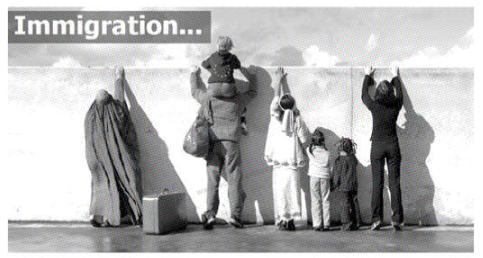
\includegraphics[width=\columnwidth]{subareas/linguagens/ingles-1.png}
\citacao{
  Your Car is German. Your Vodka is Russian. Your Pizza is Italian.
  Your Democracy is Greek. Your Coffee is Brazilian. Your Movies are
  American. Your Shirt is Indian. Your Oil is Saudi Arabian. Your
  Electronics are Chinese. Your Numbers Arabic, your Letters Latin.
  And YOU complain that YOUR Neighbor is an Immigrant?
} {
  (Adaptado de https://br.pinterest.com. Acessado em 10/06/2018.)
}

O post anterior aponta
\begin{alternativas}
  \item as vantagens da globalização para o consumidor e os problemas causados pela imigração.
  \item o impacto negativo dos processos migratórios no modo como as culturas vêm sendo globalizadas.
  \item os efeitos da globalização no nosso cotidiano e o preconceito contra imigrantes.
  \item o consumo excessivo de produtos estrangeiros no mundo capitalista contemporâneo.
\end{alternativas}

% (UNICAMP- SP - 2019)Número Original: 87Código: 6983667

\questao
\begin{center}
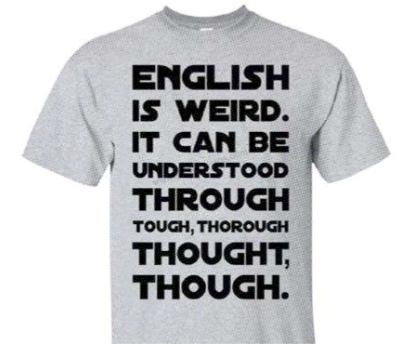
\includegraphics[width=0.6\columnwidth]{subareas/linguagens/ingles-4.png}
\end{center}
Os dizeres da camiseta:
\begin{alternativas}
  \item brincam com palavras do inglês que têm grafias e pronúncias semelhantes.
  \item criam um efeito de humor explorando a ambiguidade de certas palavras do inglês.
  \item brincam com o fato de o inglês ser uma língua irracional e incompreensível.
  \item criam um efeito de humor a partir da complexidade do sistema ortográfico do inglês.
\end{alternativas}

% (UNESP - 2021)Número Original: 27Código: 9363635

\questao
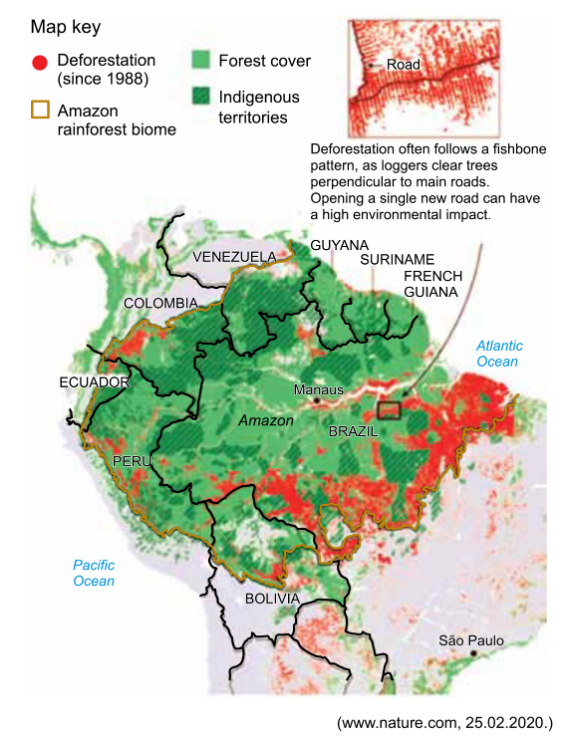
\includegraphics[width=\columnwidth]{subareas/linguagens/ingles-2.png}
The country covered by the Amazon rainforest presented in the map that displays less signs of forest clearing is:
\begin{alternativas}
  \item Ecuador.
  \item Colombia.
  \item Peru.
  \item French Guiana.
  \item Bolivia.
\end{alternativas}


% ENEM - 2021

\questao
\citacao{
  We are now a nation obsessed with the cult of celebrity. Celebrities have replaced the classic notion of the hero. But instead of being respected for talent, courage or intelligence, it is money, style and image the deciding factors in what commands respect. Image is everything. Their image is painstakingly constructed by a multitude of different image consultants to carve out the most profitable celebrity they can. Then society is right behind them, believing in everything that celebrity believes in. Companies know that people will buy a product if a celebrity has it too. It is as if the person buying the product feels that they now have some kind of connection with the celebrity and that some of their perceived happiness will now be passed onto the consumer. So to look at it one way, the cult of celebrity is really nothing more than a sophisticated marketing scheme. Celebrities though cannot be blamed for all negative aspects of society. In reality society is to blame. We are the people who seemed to have lost the ability to think for ourselves. I suppose it's easier to be told what to think, rather than challenging what we are told. The reason we are swamped by celebrity is because there is a demand for it.
} {
  Disponível em: www. pitlanemagazine.com. Acesso em: 7 dez. 2017 (adaptado).
}

O texto, que aborda questões referentes ao tema do culto à celebridade, tem o objetivo de

\begin{alternativas}
  \item destacar os méritos das celebridades.
  \item criticar o consumismo das celebridades.
  \item ressaltar a necessidade de reflexão dos fãs.
  \item culpas as celebridades pela obsessão dos fãs.
  \item valorizar o marketing pessoal das celebridades
\end{alternativas}

% [PUCPR 2003]

\questao
Supply the sentences with the correct alternative: 

\begin{enumerate}[label=\Roman*., noitemsep, topsep=1ex]
\item  This is the hardest problem \rule{1cm}{1pt} I have ever had to face. 
\item  A doctor, \rule{1cm}{1pt} patients trust him, has great responsibility. 
\item  Vesuvius, \rule{1cm}{1pt} is a lofty volcano, overlooks the Bay of Naples. 
\item  My friend Marcello, \rule{1cm}{1pt} is in hospital, is very ill. 
\item  There's something \rule{1cm}{1pt} I must tell you in confidence.
\end{enumerate}

\begin{alternativas}
  \item I. that; II. which; III. what; IV. who; V. that 
  \item I. which; II. whose; III. that; IV. whose; V. which 
  \item I. that; II. whose; III. which; IV. who; V. that 
  \item I. what; II. who; III. which; IV. that; V. what 
  \item I. that; II. whose; III. what; IV. which; V. that
\end{alternativas}

%\separador
\pagebreak
\noindent A imagem abaixo será usada nas questões \textbf{\ref{ing1}}, \textbf{\ref{ing2}} e \textbf{\ref{ing3}}.
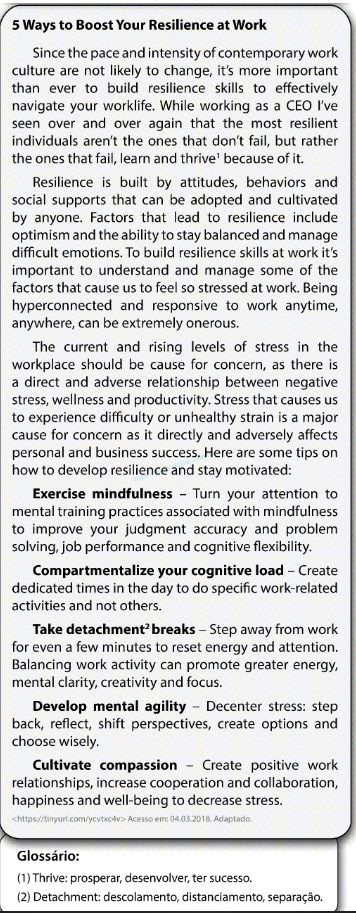
\includegraphics[width=\columnwidth]{subareas/linguagens/ingles-3.png}

\questao\label{ing1}
Segundo o texto, o crescente nível de estresse no trabalho
\begin{alternativas}
  \item deve ser motivo de preocupação pela pressão gerada.
  \item possibilita a cooperação e colaboração entre os trabalhadores.
  \item causa pressão favorável à busca por bem-estar e produtividade.
  \item estimula o trabalhador a buscar seu sucesso pessoal e profissional.
  \item cria competitividade e, consequentemente, aumenta a produtividade.
\end{alternativas}

\questao\label{ing2}
De acordo com o texto, a resiliência no mundo do trabalho
\begin{alternativas}
  \item é uma habilidade que poucas pessoas conseguem cultivar.
  \item está diretamente ligada a adversidades, causando o estresse.
  \item estabelece uma relação direta entre estresse negativo, bem-estar e produtividade.
  \item é desenvolvida com a compreensão e gerenciamento de fatores que nos causam estresse.
  \item é o resultado de um comportamento de constante conexão e disponibilidade para o trabalho.
\end{alternativas}

\questao\label{ing3}
No segundo parágrafo do texto o trecho ``... can be extremely onerous.'' refere-se a
\begin{alternativas}
  \item desenvolver a resiliência no trabalho.
  \item aumentar o nível de estresse no trabalho.
  \item estabelecer pausas excessivas durante o trabalho.
  \item compreender os fatores causadores do estresse no trabalho.
  \item estar constantemente conectado e disponível às demandas do trabalho.
\end{alternativas}


% 1.(Enem/2013)
\questao
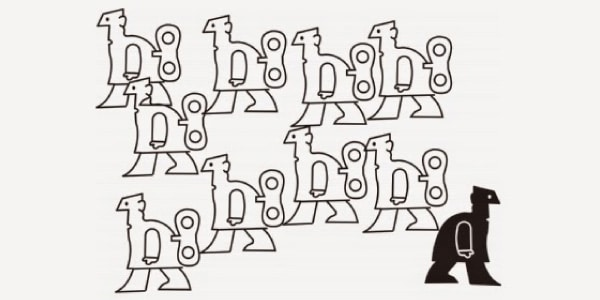
\includegraphics[width=\columnwidth]{subareas/linguagens/image3.png}
O cartum faz uma crítica social. A figura destacada está em oposição às outras e representa a
\begin{alternativas}
  \item a opressão das minorias sociais.
  \item carência de recursos tecnológicos.
  \item falta de liberdade de expressão.
  \item defesa da qualificação profissional.
\end{alternativas}

% 2.(Enem/2016)
\questao
\citacao{
  \begin{verse}
    Antiode

    Poesia, não será esse \\
    o sentido em que \\
    ainda te escrevo: \\
    flor! (Te escrevo: \\
    flor! Não uma \\
    flor, nem aquela \\
    flor-Virtude – em disfarçados urinóis). \\
    Flor é a palavra \\
    flor; verso inscrito \\
    no verso, como as \\
    manhãs no tempo. \\
    Flor é o salto \\
    da ave para o voo: \\
    o salto fora do sono \\
    quando seu tecido \\
    se rompe; é uma explosão \\
    posta a funcionar, \\
    como uma máquina, \\
    uma jarra de flores.
  \end{verse}
} {
  MELO NETO, J. C. Psicologia da composição Rio de Janeiro Nova Fronteira, 1997 (fragmento)
}
A poesia é marcada pela recriação do objeto por meio da linguagem, sem necessariamente explicá-lo. Nesse fragmento de João Cabral de Melo Neto, poeta da geração de 1945, o sujeito lírico propõe a recriação poética de
\begin{alternativas}
  \item uma palavra, a partir de imagens com as quais ela pode ser comparada, a fim de assumir novos significados.
  \item um urinol, em referência às artes visuais ligadas às vanguardas do início do século XX.
  \item uma ave, que compõe, com seus movimentos, uma imagem historicamente ligada à palavra poética.
  \item uma máquina, levando em consideração a relevância do discurso técnico-científico pós-Revolução Industrial.
  \item um tecido, visto que sua composição depende de elementos intrínsecos ao eu lírico.
\end{alternativas}

% 3.(Enem/2013)
\questao
\citacao{
  O jogo é uma atividade ou ocupação voluntária, exercida dentro de certos e determinados limites de tempo e de espaço, segundo regras livremente consentidas, mas absolutamente obrigatórias, dotado de um fim em si mesmo, acompanhado de um sentimento de tensão e de alegria e de uma consciência de ser diferente da ``vida quotidiana''.
} {
  HUIZINGA, J. Homo ludens: o jogo como elemento da cultura. São Paulo: Perspectiva, 2004.
}
Segundo o texto, o jogo comporta a possibilidade de fruição. Do ponto de vista das práticas corporais, essa fruição se estabelece por meio do(a)
\begin{alternativas}
  \item fixação de táticas, que define a padronização para maior alcance popular.
  \item competitividade, que impulsiona o interesse pelo sucesso.
  \item refinamento técnico, que gera resultados satisfatórios.
  \item caráter lúdico, que permite experiências inusitadas.
  \item uso tecnológico, que amplia as opções de lazer.
\end{alternativas}

% 4.(Enem/2014)
% 
\questao
\citacao{
  \noindent Censura moralista

  Há tempos que a leitura está em pauta. E, diz-se, em crise. Comenta-se esta crise, por exemplo, apontando a precariedade das práticas de leitura, lamentando a falta de familiaridade dos jovens com livros, reclamando da falta de bibliotecas em tantos municípios, do preço dos livros em livrarias, num nunca acabar de problemas e de carências. Mas, de um tempo para cá, pesquisas acadêmicas vêm dizendo que talvez não seja exatamente assim, que brasileiros leem, sim, só que leem livros que as pesquisas tradicionais não levam em conta. E, também de um tempo para cá, políticas educacionais têm tomado a peito investir em livros e em leitura.
} {
  LAJOLO, M. Disponível em: www.estadao.com.br. Acesso em: 2 dez. 2013 (fragmento).
}
Os falantes, nos textos que produzem, sejam orais ou escritos, posicionam-se frente a assuntos que geram consenso ou despertam polêmica. No texto, a autora
\begin{alternativas}
  \item ressalta a importância de os professores incentivarem os jovens às práticas de leitura.
  \item critica pesquisas tradicionais que atribuem a falta de leitura à precariedade de bibliotecas.
  \item rebate a ideia de que as políticas educacionais são eficazes no combate à crise de leitura.
  \item questiona a existência de uma crise de leitura com base nos dados de pesquisas acadêmicas.
  \item atribui a crise da leitura à falta de incentivos e ao desinteresse dos jovens por livros de qualidade.
\end{alternativas}

% 5.(Enem/2017)

\questao
\citacao{
  Essas moças tinham o vezo de afirmar o contrário do que desejavam. Notei a singularidade quando principiaram a elogiar o meu paletó cor de macaco. Examinavam-no sérias, achavam o pano e os aviamentos de qualidade superior, o feitio admirável. Envaideci-me: nunca havia reparado em tais vantagens. Mas os gabas se prolongaram, trouxeram-me desconfiança. Percebi afinal que elas zombavam e não me susceptibilizei. Longe disso: achei curiosa aquela maneira de falar pelo avesso, diferente das grosserias a que me habituara. Em geral me diziam com franqueza que a roupa não me assentava no corpo, sobrava nos sovacos.
} {
  RAMOS, G. Infância. Rio de Janeiro: Record, 1994.
}
Por meio de recursos linguísticos, os textos mobilizam estratégias para introduzir e retomar ideias, promovendo a progressão do tema. No fragmento transcrito, um novo aspecto do tema é introduzido pela expressão
\begin{alternativas}
  \item ``a singularidade''.
  \item ``tais vantagens''.
  \item ``os gabas''.
  \item ``Longe disso''.
  \item ``Em geral''.
\end{alternativas}
% 6.(Enem/2013)

\questao
\citacao{
  \noindent Novas tecnologias

  Atualmente, prevalece na mídia um discurso de exaltação das novas tecnologias, principalmente aquelas ligadas às atividades de telecomunicações. Expressões frequentes como ``o futuro já chegou'', ``maravilhas tecnológicas'' e ``conexão total com o mundo'',  ``fetichizam'' novos produtos, transformando-os em objetos do desejo, de consumo obrigatório. Por esse motivo carregamos hoje nos bolsos, bolsas e mochilas o ``futuro'' tão festejado. Todavia, não podemos reduzir-nos a meras vítimas de um aparelho midiático perverso, ou de um aparelho capitalista controlador. Há perversão, certamente, e controle, sem sombra de dúvida. Entretanto, desenvolvemos uma relação simbiótica de dependência mútua com os veículos de comunicação, que se estreita a cada imagem compartilhada e a cada dossiê pessoal transformado em objeto público de entretenimento. Não mais como aqueles acorrentados na caverna de Platão, somos livres para nos aprisionar, por espontânea vontade, a esta relação sadomasoquista com as estruturas midiáticas, na qual tanto controlamos quanto somos controlados.
} {
  SAMPAIO A. S. A microfísica do espetáculo. Disponível em: http://observatoriodaimprensa.com. br. Acesso em: 1 mar 2013 (adaptado).
}
Ao escrever um artigo de opinião, o produtor precisa criar uma base de orientação linguística que permita alcançar os leitores e convencê-los com relação ao ponto de vista defendido. Diante disso, nesse texto, a escolha das formas verbais em destaque objetiva
\begin{alternativas}
  \item criar relação de subordinação entre leitor e autor, já que ambos usam as novas tecnologias.
  \item enfatizar a probabilidade de que toda população brasileira esteja aprisionada às novas tecnologias.
  \item indicar, de forma clara, o ponto de vista de que hoje as pessoas são controladas pelas novas tecnologias.
  \item tornar o leitor copartícipe do ponto de vista de que ele manipula as novas tecnologias e por elas é manipulado.
  \item demonstrar ao leitor sua parcela de responsabilidade por deixar que as novas tecnologias controlem as pessoas. 
\end{alternativas}

% 7.(Enem/2013)


\questao
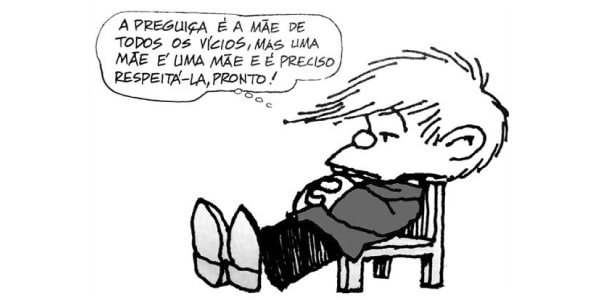
\includegraphics[width=\columnwidth]{subareas/linguagens/image2.png}
Nessa charge, o recurso morfossintático que colabora para o efeito de humor está indicado pelo(a)
\begin{alternativas}
  \item emprego de uma oração adversativa, que orienta a quebra da expectativa ao final.
  \item uso de conjunção aditiva, que cria uma relação de causa e efeito entre as ações.
  \item retomada do substantivo ``mãe'', que desfaz a ambiguidade dos sentidos a ele atribuídos.
  \item utilização da forma pronominal ``la'', que reflete um tratamento formal do filho em relação à ``mãe''.
  \item repetição da forma verbal ``é'', que reforça a relação de adição existente entre as orações.
\end{alternativas}

% 8.(Enem/2021)

\questao
\citacao{
  O documentário O menino que fez um museu, direção de Sérgio Utsch, produção independente de brasileiros e britânicos, gravado no Nordeste em 2016, mais precisamente no distrito Dom Quintino, zona rural do Crato foi premiado em Londres, pela Foreign Press Association (FPA), a associação de correspondentes estrangeiros mais antiga do mundo, fundada em 1888.

  De acordo com o diretor, O menino que fez um museu foi o único trabalho produzido por equipes fora do eixo Estados Unidos-Europa entre os finalistas. O documentário conta a história de um Brasil profundo, desconhecido até mesmo por muitos brasileiros. É apresentado com o carisma de Pedro Lucas Feitosa, 11 anos.

  Quando tinha 10 anos, Pedro Lucas criou o Museu de Luiz Gonzaga, que fica no distrito de Dom Quintino. A ideia surgiu após uma visita que o garoto fez, em 2013, quando tinha 8 anos, ao Museu do Gonzagão, em Exu, Pernambuco. Pedro decidiu criar o próprio lugar de exposição para homenagear o rei e o local escolhido foi a casa da sua bisavó já falecida, que fica ao lado da casa dele, na rua Alto de Antena.
}{}

No segundo parágrafo, uma citação afirma que o documentário "foi o único trabalho produzido por equipes fora do eixo Estados Unidos-Europa entre os finalistas". No texto, esse recurso expressa uma estratégia argumentativa que reforça a
\begin{alternativas}
  \item originalidade da iniciativa de homenagem à vida e à obra de Luiz Gonzaga
  \item falta de concorrentes ao prêmio de uma das associações mais antigas do mundo
  \item proeza da premiação de uma história ambientada no interior do Nordeste brasileiro.
  \item escassez de investimentos para a produção cinematográfica independente no país.
  \item importância da parceria entre brasileiros e britânicos para a realização das filmagens.
\end{alternativas}


% 9.(Enem/2016)
\questao
\citacao{
  Ler não é decifrar, como num jogo de adivinhações, o sentido de um texto. É, a partir do texto, ser capaz de atribuir-lhe significado, conseguir relacioná-lo a todos os outros textos significativos para cada um, reconhecer nele o tipo de leitura que o seu autor pretendia e, dono da própria vontade, entregar-se a essa leitura, ou rebelar-se contra ela, propondo uma outra não prevista.
} {
  LAJOLO, M. Do mundo da leitura para a leitura do mundo. São Paulo: Ática, 1993.
}
Nesse texto, a autora apresenta reflexões sobre o processo de produção de sentidos, valendo-se da metalinguagem. Essa função da linguagem torna-se evidente pelo fato de o texto
\begin{alternativas}
  \item ressaltar a importância da intertextualidade.
  \item propor leituras diferentes das previsíveis.
  \item apresentar o ponto de vista da autora.
  \item discorrer sobre o ato de leitura.
  \item focar a participação do leitor.
\end{alternativas}

% 10.(Enem/2016)

\questao
\textbf{TEXTO I}
\begin{center}
  \textbf{Poesia em cartaz}
\end{center}
O caminho habitual para o trabalho, aquele em que a gente já nem repara direito, pode ficar mais belo com um poema. O projeto \#UmLambePorDia nasceu desta intenção: trazer mais cor e alegria para a cidade por meio de cartazes coloridos aos estilo lambe-lambe. Quem teve a ideia foi o escritor Leonardo Beltrão, em Belo Horizonte. "Em meio a olhares cada vez mais viciados, acabamos nos esquecendo da beleza envolvida em cada esquina e no próprio poder transformador da palavra". Assim, a cada dia um cartaz é colocado por aí, para nos lembrar de reparar na cidade, na vida que corre ao redor e também em nós mesmos.

\noindent
\textbf{TEXTO II}
\par\noindent
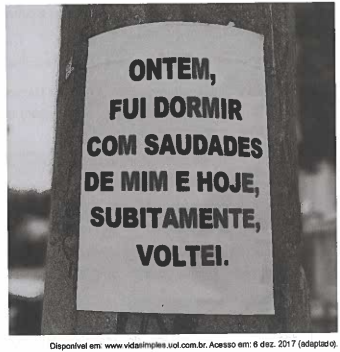
\includegraphics[width=\columnwidth]{subareas/linguagens/image1.png}

Considerando-se a função que os cartazes colados em postes normalmente exercem nas ruas das cidades grandes, esse texto evidencia a
\begin{alternativas}
  \item disseminação da arte poética em um veículo não convencional.
  \item manutenção da expectativa das pessoas ao andarem pelas ruas.
  \item necessidade de exposição de poemas pequenos em diferentes suportes.
  \item característica corriqueira do suporte lambe-lambe, muito comum nas ruas.
  \item exposição da beleza escondida das esquinas da cidade de Belo Horizonte.
\end{alternativas}

\label{last-linguagens}

%%% Local Variables:
%%% mode: latex
%%% TeX-master: "../main"
%%% End:
